\subsection{The Server}
The heard of the communication is the server. We used java\cite{java} as our programming language of choice, because of its multi platform abilities and the build in window framework of the development suit eclipse\cite{eclipse} called swt\cite{swt}. Except for one library, the RxTx-Library\cite{rxtx}, we only used basic java libraries which came by default with the eclipse IDE\cite{ide}  or alternatively the jdk7-openjdk\cite{open_jdk} package.
Provided the users connected through the interface with a serial It takes most of the information broadcasted by the panStamps\cite{panstamp} and processes them.
Provided the users connected through the interface with a serial port with the server-panStamp plugged in, the server takes the message with help of the RxTx-library\cite{rxtx} on a separate thread and passes the message, after receiving it, to the parser for processing and deciding.

\begin{figure}[ht]
\centering
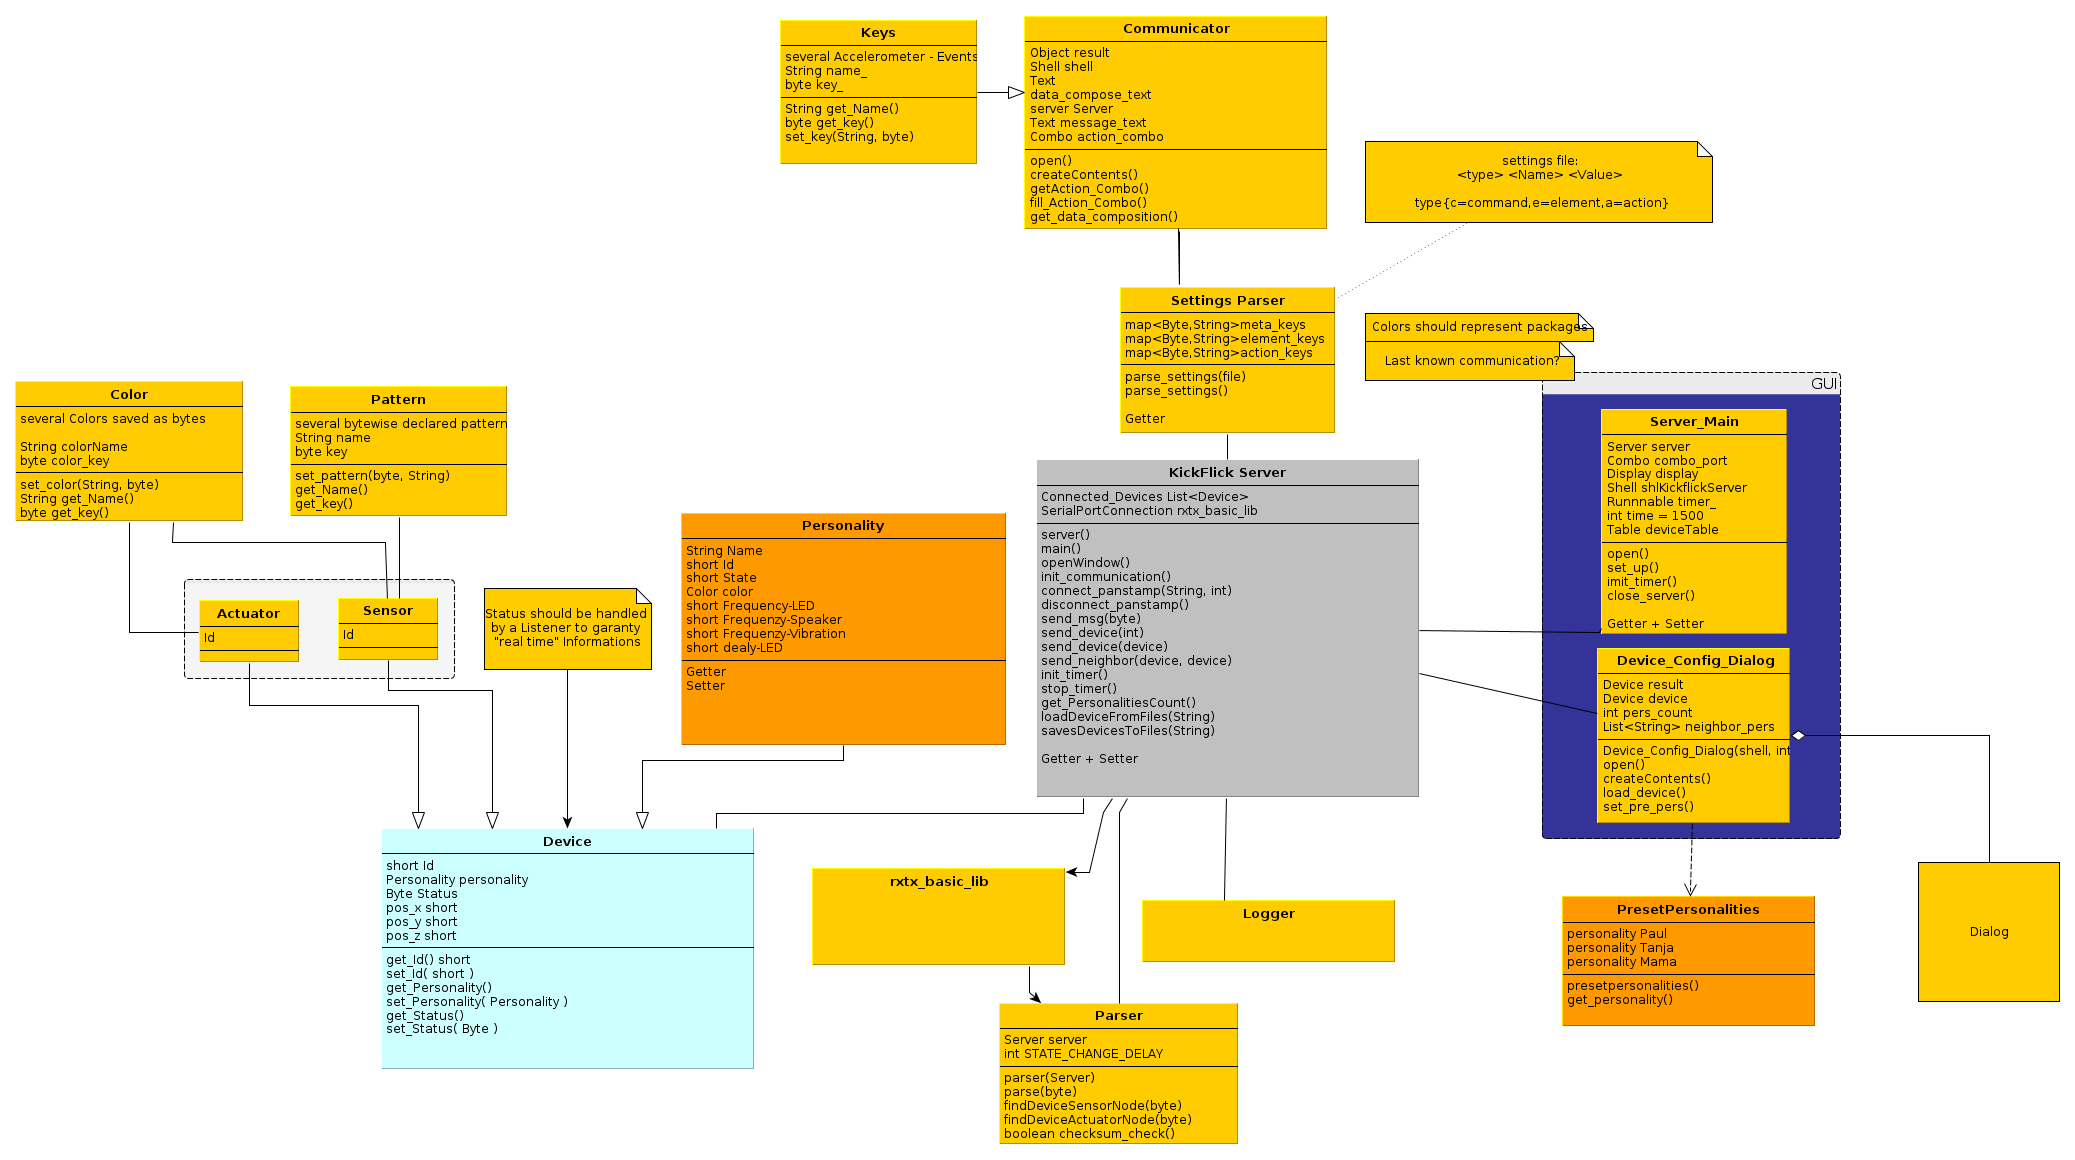
\includegraphics[width=1\textwidth]{./graph/general.eps}
\end{figure}

\subsubsection{The Parser}
The Parser takes messages in form of byte arrays with the length of four bytes. The message size was set fixed, due to a more convenient workflow and to limit the broadcasting overhead to a minimum. 
First the parser checks whether the length of the package is exactly four bytes and if the last byte, which is supposed to be a checksum summing the byte values of every other byte in the message, matches the checksum calculated by the server. If every think is correct the parser then searches for a known device in the device list of the server, if it found no match, it will create a new device with default settings. Once a device was found or created the parser begins to compare the second byte of the message for matching keys stored by the server. First all system\_keys will be compared. For example if the received message contains a ''52'' as second byte, the parser will then recognize this as the ''the battery is low'' key and will toggle the boolean value battery\_low of the device to true. 
If no system key matched with the received one, the parser then checks the reaction keys of the device itself. This check only happens if the device it not currently engaged in a neighborhood relationship with another device and if the time of the last received state changing message lays back a certain time. For this checking and comparing procedure the device owns a map with all reaction keys stored to it and a associated boolean value, representing the choice of ignoring or reacting to the received key. If a appropriate key was found and according to the boolean value a reaction should happen, then the state of the devices personality will be increased and the new information about the pattern and both colours will be send to the server-panStamp using the RxTx-library.

\subsubsection{Device and Personality Structure}
The server itself and the according class holds a list of all known devices. Every lookup action depends on this list. The device class itself holds a instance of the personality class.
Devices can be seen as a representation of the hardware devices with the two panStamps in them. It refers to the hardware and therefor stores the Id's of the panStamps and timestamps of the last received message either one of the hardware device panStamps, a second timestamp of the last state change and a third timestamp of the last ''neighborhood meeting''. All those information are accessible through ''get'' functions as well as mostly modifiable through ''set'' functions.

The personality class stores information about the states of the personality and the according patterns and colors. This class also provides ''get'' and ''set'' functions to retrieve or change values. Additionally the personality class stores map object of all known personalities and the appropriate response in form of pattern and colors to every possible neighbor. If the device and therefor the personality encounter a unknown personality as a neighbor a default response will be send. 
The neighbor map provides the ability to set reactions to neighbor personality, even if they don't exist yet.

To get the server and the project running without setting up every single device by hand a enumeration for pre defined personalities was created. One can select between each of those personalities. Once a pre defined personality is selected, the previous personality of the current device will be overwritten. This approach saves time.

\subsubsection{Key Structure}
During the development we thought of keys, single byte values, to represent commands, messages, patterns and colors. To store these keys several enumerations were created to seperate related keys with their name and value depending on their usage.
We divided the keys in enumerations:
\begin{itemize}
    \item system
    \begin{itemize}
         \item stores basic keys for transmitting status information (e.g. ''low battery'')
    \end{itemize}
    \item color
    \begin{itemize}
        \item stores byte values for every color hard coded to the actuator panStamp of the hardware device
    \end{itemize}
    \item pattern
    \begin{itemize}
        \item stores byte values for every pattern hard coded to the actuator panStamp of the hardware device
    \end{itemize}
    \item key
    \begin{itemize}
        \item stores byte values for every possible action happening to the hardware device
    \end{itemize}
\end{itemize} 

Every class or function referring to those values calls only the enumeration item by its name. The advantage of this approach is easier changing of single values as well as a quicker overview.
